\section{Results}

% benchmarks used
\subsection{Naturalistic task}
The evaluation of the model ability to construct and utilize a cognitive map was defined as the total rewards collected during several rewards trials in different environments.
The protocol was inspired by the behaviour of animals who are end up in a new territory in search for food in various locations.

The testing environments varied in layout, determined by the position and number of walls.

First there was the exploration phase, in which the agent was placed in a random location and let roam through a pseudo-random walk for 5000 steps. Depending on environment layout, the formed map was more or less matching the the actual topology.
Then the exploitation phase began, in which a circle the 5\% of the total are was designated to provide a binary reward $R\sim \mathcal{B}(p_{r})$ drawn from a Bernoully with probability $p_{r}$.
When the reward was successfully fetched, the agent was teleported to a random location in the environment.
Further, in order to mimic the depletion of a food source the reward area was modeled with as leaky variable $\dot{v}_{r}=(E_{r}-v_{r})/\tau_{r} + R$, and its location moved whenever its level went below a threshold $v_{r}<\theta_{r}$.

\hfill \break
The optimization of the parameters of the model was carried out using the Covariance-Matrix Adaptation evolutionary strategy (CMA-ES) \cite{igelCovarianceMatrixAdaptation2007} with a population of 256 individuals for 100 generations.


\subsection{Performance over different environments}
The best model resulting from evolution reached solid navigation and adaptation skills. Within the limits imposed by the rudimentary exploration policy based on random walks, the agent was able to visit a significant portion of the environment during exploration, and tune its modulatory system to craft cognitive maps useful during exploitation.

In figure \ref{fig:results_1} we can see the cognitive maps formed by the agent in three different environments.
In plot \ref{fig:results_1}-\textbf{a} it is reported a linear track with wide margins, represented in terms of four layers: the nodes of the fine-grained place cells (top), the graph of the coarse-grained place cells (center-top), the boundary-tagged place cells (center-bottom), and the reward-tagged place cells (bottom).
The overlap of these last three representations is what we refer to as the cognitive map, since these are the layers providing the main information used during goal planning.
In plot \ref{fig:results_1}-\textbf{b} and \ref{fig:results_1}-\textbf{c} we can see the cognitive maps formed in a square environment without and with internal walls, respectively.

In red is indicated the trajectory of the agent, and notable it is the greater number of lines crossing into the rewarding zone, in green.
The agent's planned path is shown in grey, highlighting how it dodges the walls and go straight to the goal.

\begin{figure}[h]
    \centering
    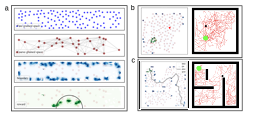
\includegraphics[width=0.9\textwidth]{figures/results_1.png}
    \caption{\textsc{Cognitive maps and agent behaviour} - \textbf{a}: \textit{place cells (PCs) over a rectangular environment, where the top plot report the node centers of the fine grained PCs, the top-center plot the node centers of coarse grained PCs together with their edges, the bottom-center
        instead shows the activity of the PCs tagged with the boundary neuromodulator over the coarse grained PCs, while the bottom plot shows the same but with the PCs tagged by the reward neuromodulator; the semicircle corresponds to the reward area} -
    \textbf{b}: \textit{square environment, the right plot is the agent's trajectory (red) and reward area (green), the left plot si the \textit{cognitive map}, defined as overlay of the coarse-grain PCs, boundary and reward-sensitive PCs.} -
    \textbf{c}: \textit{square environment with internal walls, the right and left plot as before, but with the addition of the path planned by the agent to reach the target (grey)}}
    \label{fig:results_1}
\end{figure}


\subsection{Modulation of cell density affects performance}
















